\documentclass{beamer}
\usetheme{Madrid}
\usepackage{graphics}

\begin{document}
\title{Game of Life 2D}
\author{Federica Amato, Andrea Bonandin}
\date{21 February 2017}

\begin{frame}
	\begin{center}
		\Large{University of Pavia \\
		Advanced Computer Architecture}
	\end{center}
	\titlepage
\end{frame}

\section{Introduction}
\begin{frame}
	\frametitle{Introduction}
	\begin{itemize}
		\item Solution of the mystery of self-reproduction in cellular automata;
		\item Collection of cells on a grid;
		\item Set of rules for cells' evolution.
	\end{itemize}
	\vfill
	\begin{columns}
		\column{0.9\textwidth}
		\begin{block}{Conway's Game of Life}
			\begin{itemize}
				\item 2-dimensional cellular automaton;
				\item Zero-player game;
				\item Possibility to create several patterns;
				\item States of a population: $0 \rightarrow dead$, $1 \rightarrow alive$.
			\end{itemize}
		\end{block}
	\end{columns}
\end{frame}

\section{Transition Rules}
\begin{frame}
	\frametitle{Conway's Game of Life - Transition Rules}
	\begin{itemize}
		\item With zero or one bordering member alive in a cell's neighborhood, death occurs due to loneliness;
		\item With two or three members alive in the neighborhood, there is no change to an alive member;
		\item If a dead member's neighborhood consists of three live members, a new member is born ($0 \rightarrow 1$);
		\item If a live member's neighborhood consists of more than three live members, it will die due to overpopulation.
	\end{itemize}
\end{frame}

\section{Serial Code Analysis}
\begin{frame}
	\frametitle{Serial Code Analysis}
	\begin{minipage}{0.6\textwidth}
		\begin{itemize}
			\item The universe of the Game is represented by a rectangular grid;
			\item Toroidal boundary conditions to reduce errors at the edges;
			\item Matrices transformed in 1-D array.
		\end{itemize}
		\begin{columns}
			\column{0.9\textwidth}
			\begin{block}{Core functions}
				\begin{itemize}
					\item \textit{init}: it initializes the grid of the Game and the boundaries;\\
					\item \textit{evolve}: it updates boundary conditions and applies transition rules;\\
					\item \textit{update}: it swaps the previous state with the one.
				\end{itemize}
			\end{block}
		\end{columns}
	\end{minipage}%
	\begin{minipage}{0.4\textwidth}
		\begin{figure}
			\centering
			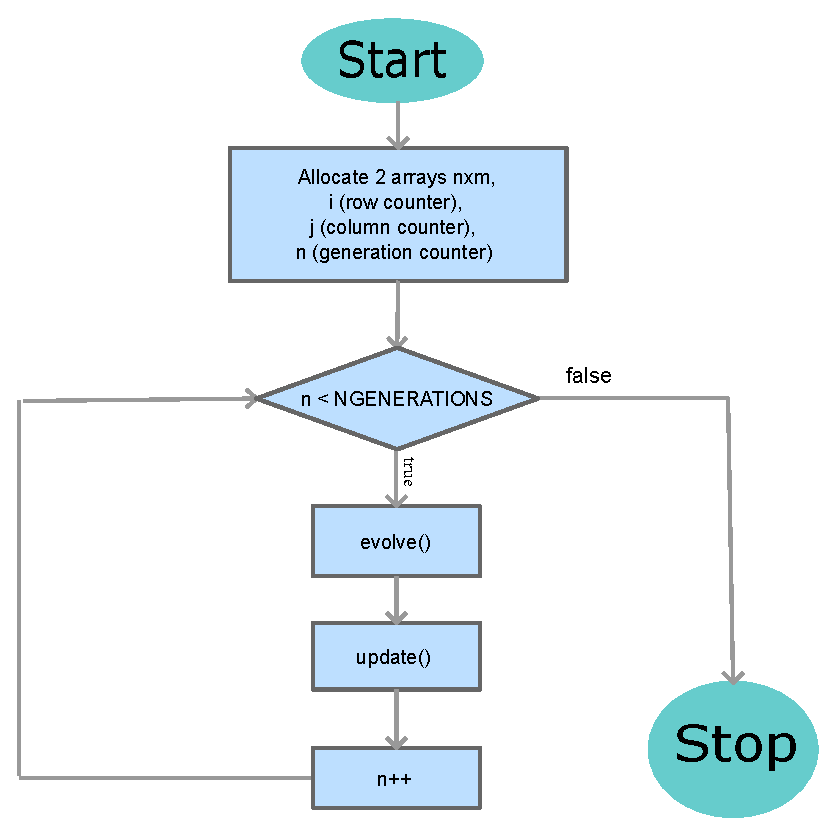
\includegraphics[width=\linewidth]{../report/chart.eps}
		\end{figure}
	\end{minipage}
\end{frame}

\section{Processor used}
\begin{frame}
	\frametitle{\emph{Intel Core i5-3230M} Processor}
	\begin{figure}
		\centering
		
\includegraphics[scale=0.2]{intel_i5.png}
	\end{figure}
	\begin{columns}
		\column{0.7\textwidth}
		\begin{block}{Processor's Characteristics}
			\begin{itemize}
				\item 2 physical cores;
				\item 4 logic cores;
				\item Frequency: 2.60 GHz;
				\item 3-level cache.
			\end{itemize}
		\end{block}
	\end{columns}
\end{frame}

\section{OpenMP Parallel Implementation}
\begin{frame}
	\frametitle{OpenMP Parallel Implementation}
	\begin{itemize}
		\item Two nested cycles in every function: parallelized the external cycle;
		\item No complex calculus;
		\item Speedup given by evolving more rows at the same time.
	\end{itemize}
	\vfill
	\begin{columns}
		\column{0.9\textwidth}
		\begin{block}{Versions}
			\begin{itemize}
				\item \emph{parallel1.c}: one parallel region in every parallelized function, static scheduling;
				\item \emph{parallel2.c}: only one parallel region, static scheduling;
				\item \emph{parallel3.c}: one parallel region, dynamic scheduling.
			\end{itemize}
		\end{block}
	\end{columns}
\end{frame}

\section{Performance's Measurements}
\begin{frame}
	\frametitle{Amdahl's Law}
	\begin{columns}
		\column{0.9\textwidth}
		\begin{block}{}
			\begin{itemize}
				\item Theoretical speedup: $S_{o} = \frac{1}{(1-f) + \frac{f}{N} + H(N)} = 2$;
				\item Hyper-threading case: $S_{HT} = \frac{1}{(1-f) + 0,67*(\frac{f}{N}) + H(N)} = 2.13$.
			\end{itemize}
		\end{block}
	\end{columns}
	\vfill
	\begin{itemize}
		\item $f = 1$, fraction of parallelized code;
		\item $N = 2$ and $H(N) = 0$ in $S_{o}$;
		\item $N = 4$ and $H(N) = 0.3$ in $S_{HT}$.
	\end{itemize}
\end{frame}

\section{Performance's Measurements}
\begin{frame}
	\frametitle{Performance's Measurements}
	\begin{figure}
		\centering
		\begin{minipage}{0.5\textwidth}
			\centering
			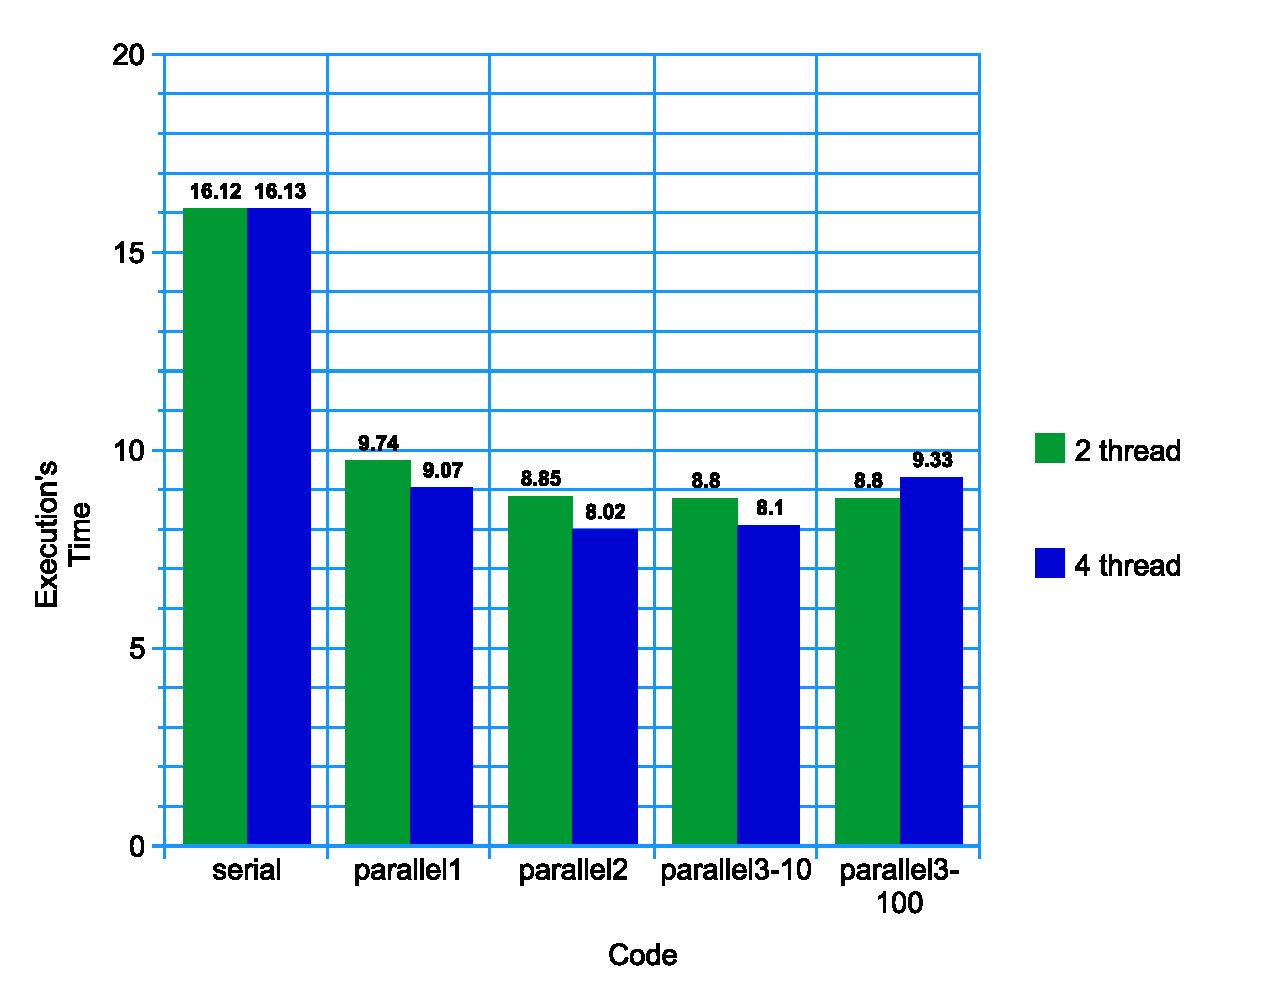
\includegraphics[width=\linewidth]{../report/graph.eps}
			\caption{$1000$ generations, $1000x1000$ grid}
		\end{minipage}%
		\begin{minipage}{0.5\textwidth}
			\centering
			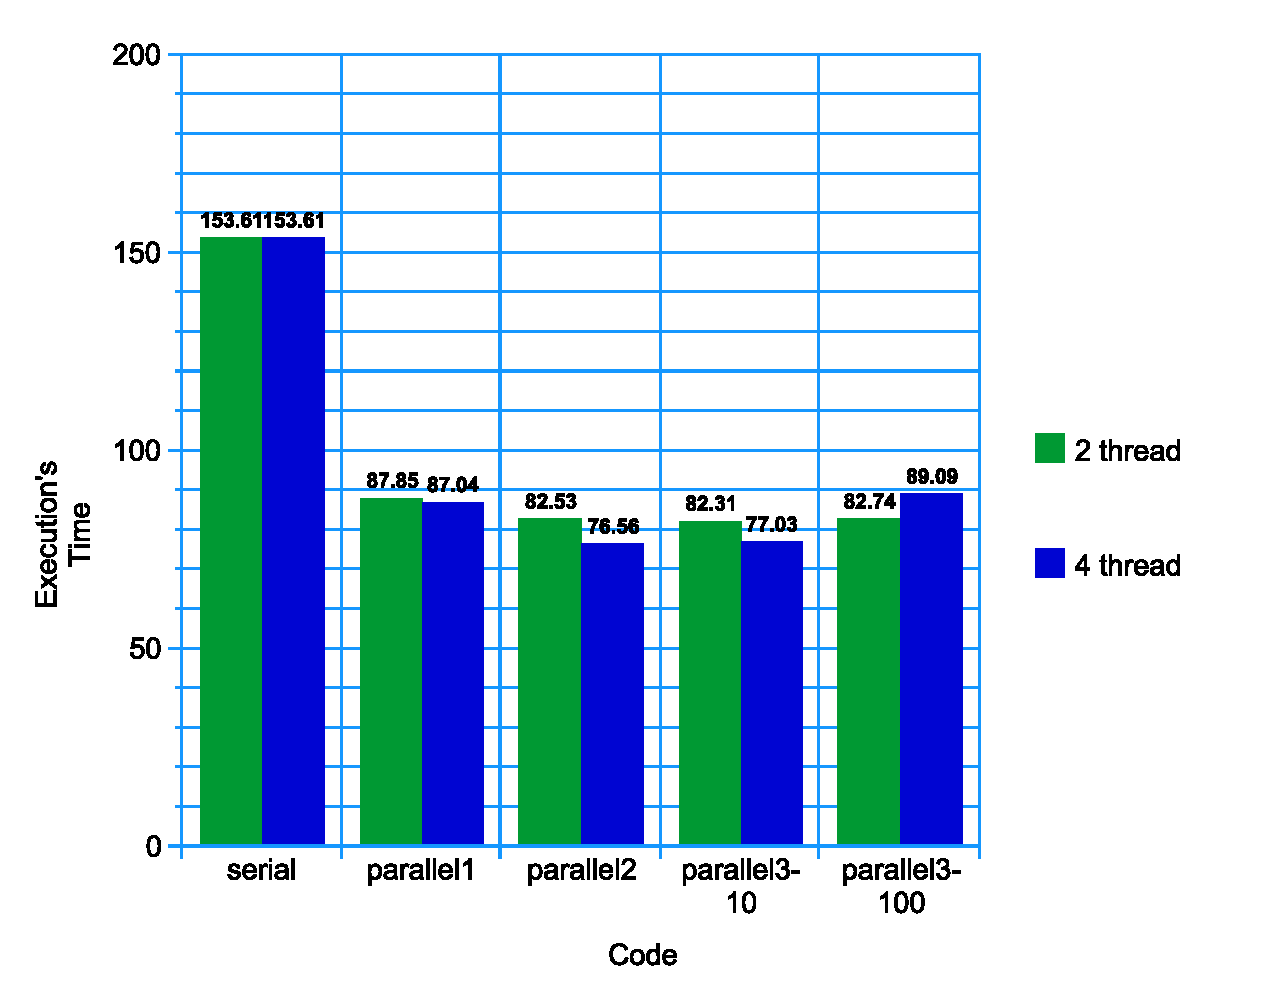
\includegraphics[width=\linewidth]{../report/1000-10000.eps}
			\caption{$10000$ generations, $1000x1000$ grid}
		\end{minipage}
	\end{figure}
\end{frame}

\section{Performance's Measurements}
\begin{frame}
	\frametitle{Performance's Measurements}
	\begin{figure}
		\centering
		\begin{minipage}{0.5\textwidth}
			\centering
			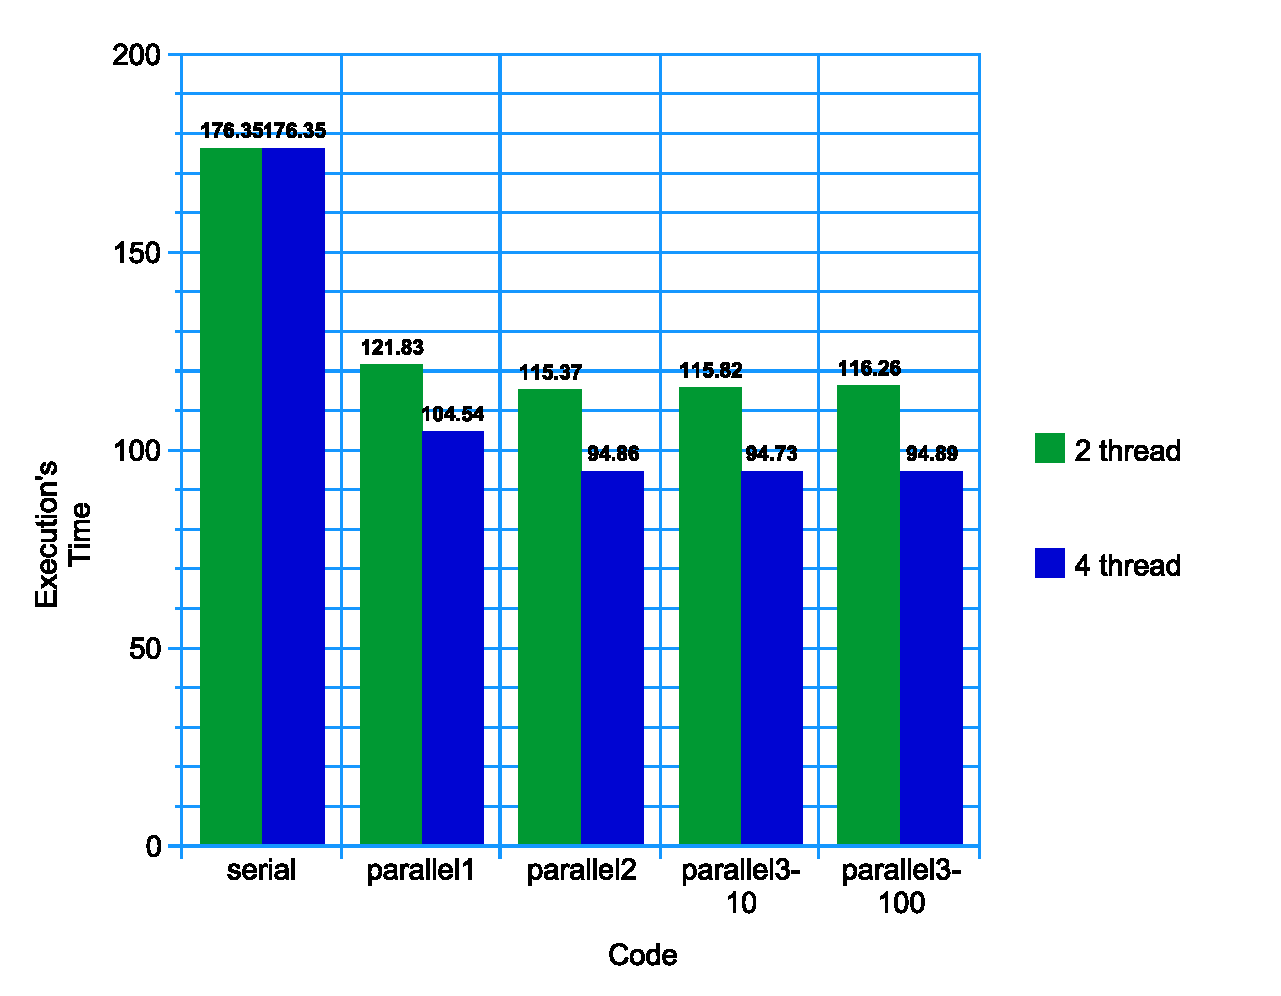
\includegraphics[width=\linewidth]{../report/10000-100.eps}
			\caption{$100$ generations, $10000x10000$ grid}
		\end{minipage}%
		\begin{minipage}{0.5\textwidth}
			\centering
			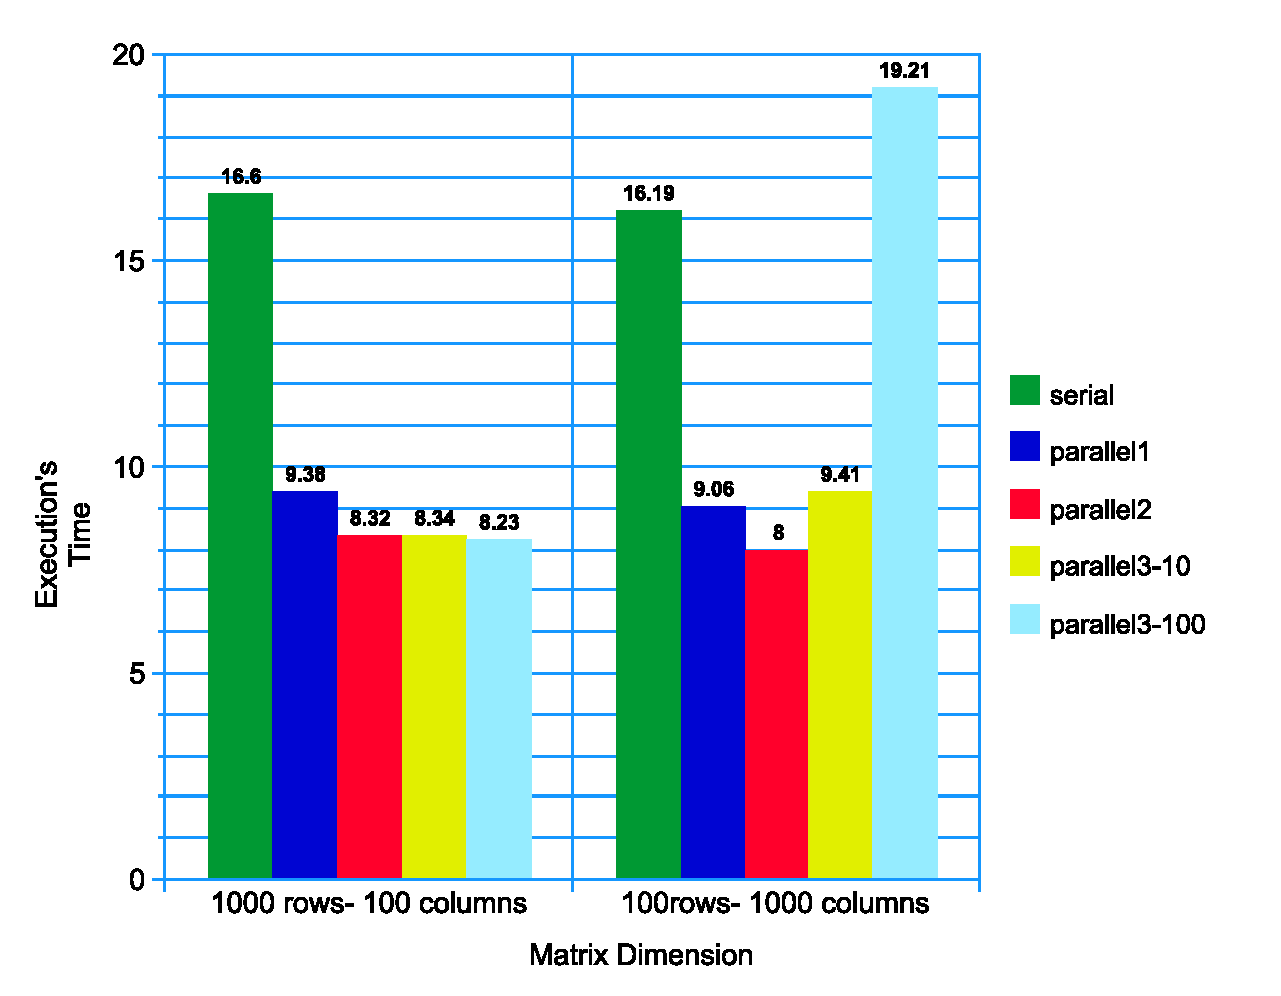
\includegraphics[width=\linewidth]{../report/matdim.eps}
			\caption{$1000$ generations, rectangular grid}
		\end{minipage}
	\end{figure}
\end{frame}

\section{Speedup}
\begin{frame}
	\frametitle{Speedup}
	\begin{figure}
		\centering
		\begin{minipage}{0.5\textwidth}
			\centering
			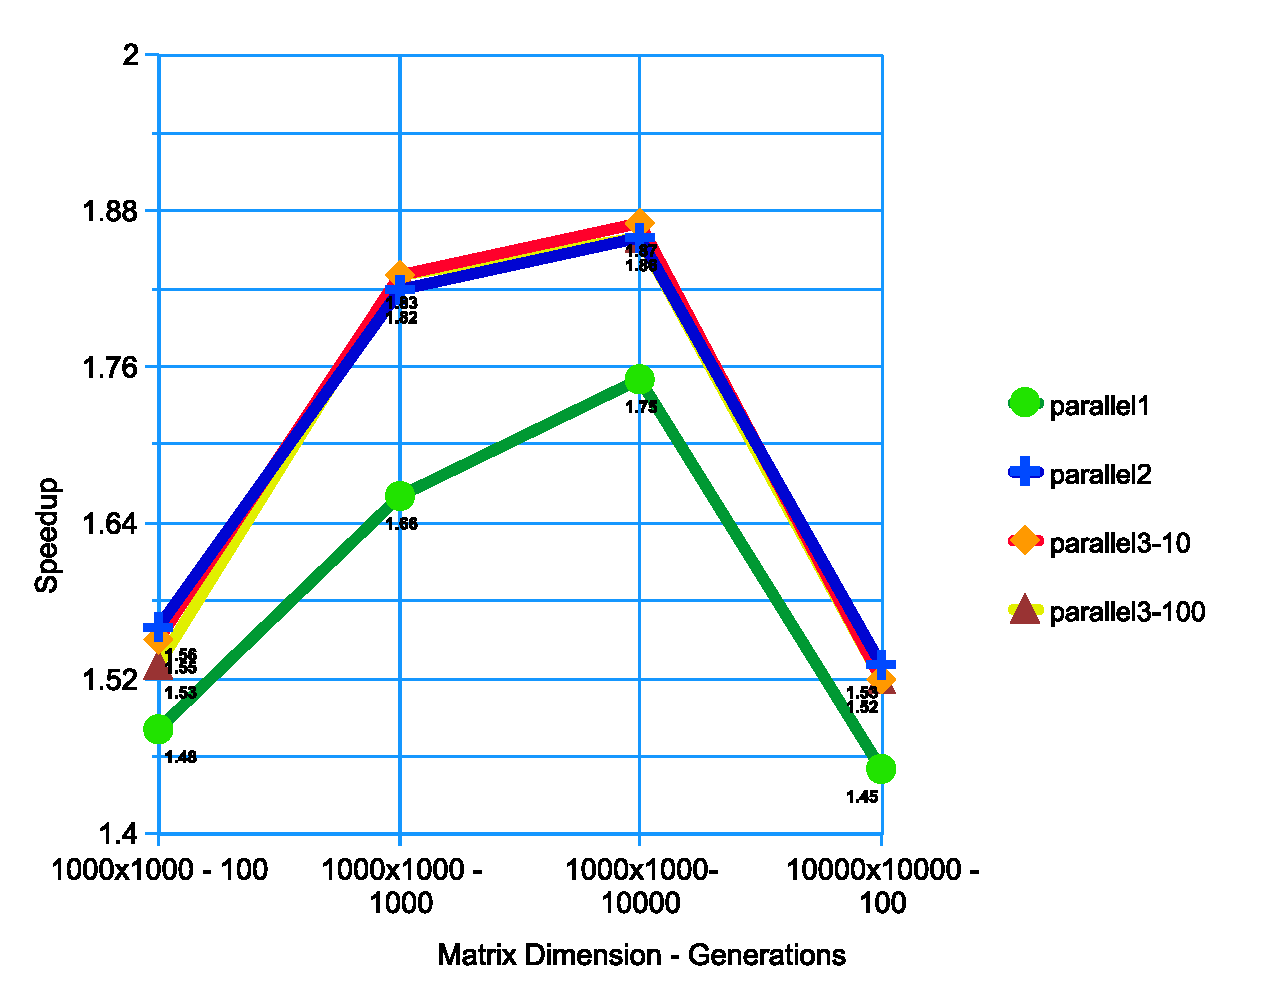
\includegraphics[width=\linewidth]{../report/2.eps}
			\caption{Speedup with 2 threads}
		\end{minipage}%
		\begin{minipage}{0.5\textwidth}
			\centering
			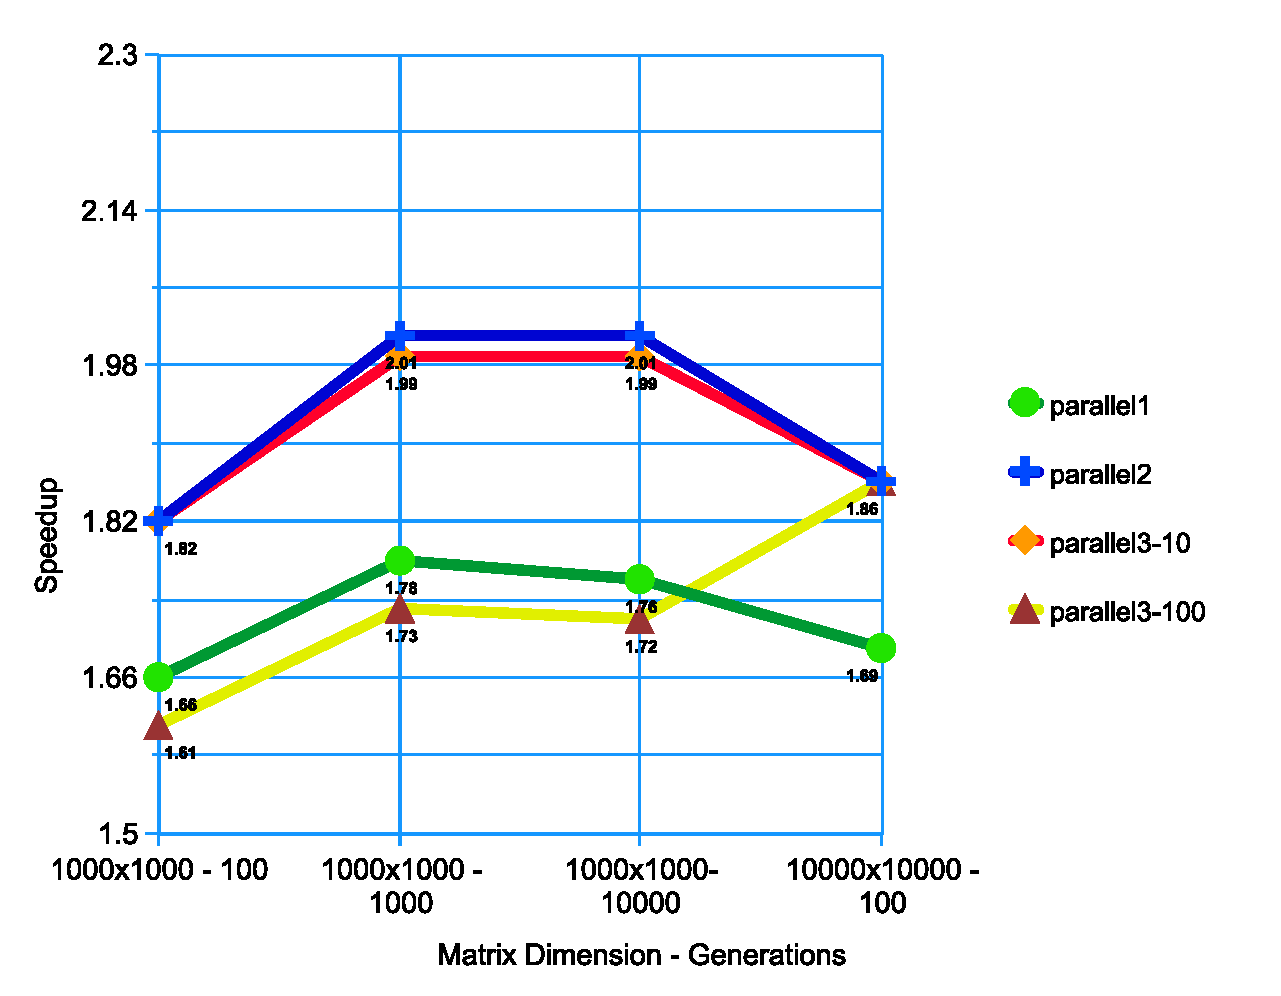
\includegraphics[width=\linewidth]{../report/4.eps}
			\caption{Speedup with 4 threads}
		\end{minipage}
	\end{figure}
\end{frame}

\section{Conclusion}
\begin{frame}
	\frametitle{Conclusion}
	\begin{itemize}
		\item We began with a serial algorithm using a matrix and without functions;
		\item We transformed the matrix into a 1-D array and we wrote three core functions;
		\item We studied the available parallelism and we proposed three parallel implementations;
		\item We tried all the versions on Intel Core i5-3230M using two and four threads;
		\item We found that the best proposal is the version with one parallel region, static scheduling and four threads.
	\end{itemize}
\end{frame}

\end{document}
